\documentclass[11pt,a4paper]{article}

% ---------------------------------------------------------------------------
% Exact interfaces for modular autocatalytic reaction networks:
% amplification prices, catalyst-aware cores, degradation onset,
% and boundary traces.
%
% Author metadata: set the three macros below before submission.
% ---------------------------------------------------------------------------
\newcommand{\PaperAuthor}{Anonymous manuscript}
\newcommand{\PaperAffiliation}{}
\newcommand{\PaperDate}{September 7, 2026}

\usepackage[T1]{fontenc}
\usepackage[utf8]{inputenc}
\usepackage{lmodern}
\usepackage{microtype}
\usepackage[a4paper,margin=1.05in]{geometry}
\usepackage{amsmath,amssymb,amsthm,mathtools}
\usepackage{booktabs}
\usepackage{array}
\usepackage{enumitem}
\usepackage{xcolor}
\usepackage{graphicx}
\usepackage{tikz}
\usetikzlibrary{arrows.meta,positioning,calc,shapes.geometric}
\usepackage{listings}
\usepackage[obeyspaces,spaces]{url}
\usepackage[numbers,sort&compress]{natbib}
\usepackage[colorlinks=true,linkcolor=blue!55!black,citecolor=blue!55!black,urlcolor=blue!55!black]{hyperref}

\DeclareUrlCommand\lean{\urlstyle{tt}}

\setlist{itemsep=2pt,topsep=3pt}
\setlength{\emergencystretch}{1.5em}

\theoremstyle{plain}
\newtheorem{theorem}{Theorem}[section]
\newtheorem{proposition}[theorem]{Proposition}
\newtheorem{lemma}[theorem]{Lemma}
\newtheorem{corollary}[theorem]{Corollary}
\theoremstyle{definition}
\newtheorem{definition}[theorem]{Definition}
\newtheorem{example}[theorem]{Example}
\newtheorem{construction}[theorem]{Construction}
\theoremstyle{remark}
\newtheorem{remark}[theorem]{Remark}
\newtheorem{nonclaim}[theorem]{Non-claim}

\lstdefinelanguage{Lean}{
  morekeywords={theorem,def,structure,inductive,namespace,end,import,by,intro,exact,constructor,refine,where,abbrev,noncomputable,rintro,simpa,using,let,have,fun,if,then,else,match,with},
  sensitive=true,
  morecomment=[l]{--},
  morestring=[b]",
}
\lstset{
  language=Lean,
  basicstyle=\ttfamily\small,
  keywordstyle=\bfseries,
  commentstyle=\itshape\color{black!60},
  columns=fullflexible,
  keepspaces=true,
  breaklines=true,
  frame=single,
  framerule=0.3pt,
  xleftmargin=1em,
  xrightmargin=1em,
  extendedchars=true,
  literate={≤}{{$\le$}}1 {≥}{{$\ge$}}1 {ℕ}{{$\mathbb{N}$}}1 {ℝ}{{$\mathbb{R}$}}1 {ℚ}{{$\mathbb{Q}$}}1 {→}{{$\to$}}1 {∀}{{$\forall$}}1 {∃}{{$\exists$}}1 {≠}{{$\neq$}}1 {∧}{{$\wedge$}}1 {¬}{{$\neg$}}1 {↔}{{$\leftrightarrow$}}1 {∑}{{$\sum$}}1 {∏}{{$\prod$}}1 {₀}{{$_0$}}1 {₁}{{$_1$}}1 {₂}{{$_2$}}1 {⟨}{{$\langle$}}1 {⟩}{{$\rangle$}}1 {∈}{{$\in$}}1 {∉}{{$\notin$}}1 {·}{{$\cdot$}}1 {α}{{$\alpha$}}1 {β}{{$\beta$}}1 {μ}{{$\mu$}}1 {λ}{{$\lambda$}}1 {θ}{{$\theta$}}1 {⊆}{{$\subseteq$}}1 {⊕}{{$\oplus$}}1 {×}{{$\times$}}1 {∆}{{$\triangle$}}1 {≃}{{$\simeq$}}1 {∩}{{$\cap$}}1 {∪}{{$\cup$}}1 {⦃}{{$\{\!\{$}}1 {⦄}{{$\}\!\}$}}1 {ι}{{$\iota$}}1 {κ}{{$\kappa$}}1 {ρ}{{$\rho$}}1 {σ}{{$\sigma$}}1
}

\newcommand{\R}{\mathbb{R}}
\newcommand{\N}{\mathbb{N}}
\newcommand{\Q}{\mathbb{Q}}
\newcommand{\C}{\mathbb{C}}
\newcommand{\Tr}{\operatorname{Tr}}
\newcommand{\Feas}{\mathsf{Feas}}
\newcommand{\Diag}{\operatorname{Diag}}
\newcommand{\spb}{s}
\newcommand{\MPAC}{\mathsf{MultiPAC}}
\newcommand{\MCAC}{\mathsf{MultiCAC}}
\newcommand{\DIR}{\mathsf{Dir}}
\newcommand{\LCC}{\mathsf{LinCx}}
\newcommand{\Tp}{^{\mathsf T}}
\newcommand{\ie}{i.e.}

\title{Exact interfaces for modular autocatalytic reaction networks:\\
amplification prices, catalyst-aware cores, degradation onset,\\ and boundary traces}
\author{\PaperAuthor\\ \PaperAffiliation}
\date{\PaperDate}

\begin{document}
\maketitle

\begin{abstract}
Modular reasoning about an autocatalytic reaction network is trustworthy only when the environment cannot exploit information that a module summary discarded. We develop, and verify in Lean~4, a layered theory of \emph{exact interfaces} for finite reaction networks with explicit catalysis. Three foundation results each identify the smallest object that composes. (i)~For the maximum amplification factor (MAF), the compositional invariant is not the scalar optimum but the threshold-indexed family of strict species-price certificates; reaction addition, species aggregation, disjoint union, and shared-species coupling act on these price cones by exact set operations, and a two-species example with MAF values $2,2,2,4$ shows that no scalar rule can exist. (ii)~Autocatalytic child-selection cores of a network with explicit catalysis are recovered exactly from its ordinary cores: a target core differs from a vertex-contained ordinary anchor by a vertex-disjoint pack of alternating matching-exchange paths, and an executable enumerator built on this fact returns precisely the child-selection cores without traversing the ambient edge powerset. (iii)~For species-specific degradation at diluted onset, the growth, critical, and extinction regions of the degradation orthant are exactly the projective images $d\lessgtr Av/v$ of positive compositions $v$, with the Perron mode constructed rather than assumed, and a finite actuator support can extinguish the system precisely when the unactuated principal block already admits a strict extinction certificate.

Interactions between factors of a source network are then organised on a typed factor--species incidence graph: amplification synergy forces a signed cycle, fixed-threshold feasibility is exactly a disjunction over factors on an incidence forest, and degradation loads of independent branches add at a shared root, so that two individually extinct branches can jointly grow. Finally we define the exact boundary trace of a module, prove that trace equality is precisely indistinguishability by every boundary context, characterise when a coarser summary is safe (injectivity on the realized traces), and give an exact junction-tree message theorem in which running intersection together with a scope-extensionality condition repairs otherwise invalid existential witness gluing; separator width bounds message arity. The MAF price-cone profile, a thermodynamic interval interface, and a finite Type-II passive tail are exact interfaces; the scalar MAF and two thermodynamic verdict vectors are certified information losses. Every stated result is compiled with warnings treated as errors in a frozen Lean~4.30 / Mathlib environment.
\end{abstract}

\noindent\textbf{Keywords.} autocatalytic networks; RAF sets; maximum amplification factor; autocatalytic cores; explicit catalysis; Metzler matrices; degradation; boundary trace; contextual equivalence; junction tree; separator width; Lean~4.

\section{Introduction}\label{sec:intro}

\subsection{The problem}

Autocatalytic reaction networks are studied through several structural lenses: reflexively autocatalytic and food-generated (RAF) sets \cite{kauffman1986,hordijk2004,hordijk2014,steel2019}, stoichiometric autocatalytic motifs and cores \cite{blokhuis2020,golnik2026cores,golnik2026bridging}, diluted-onset dynamical autocatalysis \cite{unterberger2022,nandan2026}, growth bounds such as the maximum amplification factor \cite{gagrani2026maf}, and thermodynamic realizability of cycles \cite{kosc2025}. In each lens a natural engineering question arises: if a network is assembled from modules, which module data suffice to predict the behaviour of the assembly?

The question is harder than it looks because the lenses expose different boundary data. A structural verdict, a productive flux, a spectral sign, and a thermodynamic current pattern are all summaries, and a convenient summary can agree for two isolated modules while a shared partner separates them. Three concrete phenomena drove this work.
\begin{itemize}
\item Two two-species networks with the same maximum amplification factor $2$ have parallel compositions with a common partner whose amplification factors are $2$ and $4$ (Theorem~\ref{thm:scalar-noncomp}). The scalar loses a \emph{direction}.
\item An ordinary autocatalytic core contained in a larger autocatalytic child selection need not use the same reactant matching edges (Example~\ref{ex:golnik33}). Descending along matching edges is wrong; descending along supports is right.
\item A single degraded branch coupled to a shared root may be extinct while two copies of it coupled to the same root grow (Example~\ref{ex:star}). Degradation composition is additive, not maximum-like.
\end{itemize}
Each phenomenon is an instance of one lesson: identify the smallest certificate profile that is functorial under the operations of interest, and prove exact laws on that profile before extracting scalars.

\subsection{Contributions}

The paper is organised as three foundation layers, an interaction layer, and a general interface theory. All results are formalised; Section~\ref{sec:verification} lists the terminal Lean declarations and receipts.

\begin{enumerate}[label=\textbf{(\Roman*)}]
\item \textbf{Amplification prices} (Section~\ref{sec:maf}). Threshold feasibility $\exists x\ge 0,\,x\ne 0,\ Bx\ge qAx$ is dual, by a strict finite Gordan alternative, to the nonemptiness of a strict price cone $D_N(q)$. For an attained MAF $\alpha$ one has $\alpha<q\iff D_N(q)\neq\emptyset$. Reaction addition intersects $D_N(q)$ with an open half-space, aggregation retains nonnegative lifts, disjoint union gives $\max$, and shared-species coupling intersects price cones. Equality versus strict increase of the MAF is exactly survival versus disappearance of prices above the old threshold. The scalar MAF is provably noncompositional.
\item \textbf{Catalyst-aware cores} (Section~\ref{sec:cs}). For a finite network with explicit catalysis, every autocatalytic child-selection edge set is reconstructed from a vertex-contained ordinary core by toggling a vertex-disjoint pack of alternating matching-exchange paths with external endpoints of opposite type; unique matching of the anchor excludes alternating cycles. An executable enumerator that generates only such packs, filters with proof-carrying rational certificates, and takes strict-subset minima returns exactly the child-selection cores of Golnik et al.~\cite{golnik2026cores}, Definition~3.4.
\item \textbf{Degradation onset} (Section~\ref{sec:deg}). For a diluted unary source model whose reaction graph is strongly connected, and for every nonnegative species-wise degradation $d$, the sign of the real spectral bound of $A-\Diag(d)$ is characterised by strict positive certificates, equivalently by the projective inequalities $d< Av/v$, $d=Av/v$, $Av/v<d$. The Perron mode is constructed from a finite-dimensional Schauder fixed point. Finite supported degradation on an actuator set $S$ can extinguish the system iff the unactuated principal block admits a strict extinction certificate.
\item \textbf{Factor interactions} (Section~\ref{sec:cic}). For an ownership factorization of a source network, amplification feasibility that no single active factor achieves alone forces a signed cycle in the typed factor--species incidence graph; on an incidence forest, global fixed-threshold feasibility is exactly the disjunction of factor feasibilities and the attained MAF is the maximum of factor MAFs. For a degradation star, an inverse-free Schur elimination shows that branch loads add at the root and the sign of the resulting scalar is the sign of the real spectral bound.
\item \textbf{Exact boundary traces} (Section~\ref{sec:trace}). The trace of a boundary model is the existential projection of its valid internal witnesses. Trace equality is equivalent to indistinguishability by every boundary context, with singleton contexts sufficing for the converse. A summary of the trace is contextually sufficient iff it is injective on the realized traces. A loss witness refutes sufficiency. The literal source feasibility of an ownership factorization is an exact trace.
\item \textbf{Bounded-width composition} (Section~\ref{sec:junction}). On a rooted join tree satisfying running intersection and local scope extensionality, the recursive separator message equals the one-global-assignment semantics at every node; hence separator messages are contextually substitutable, a certificate checker is sound with message arity bounded by separator width, elimination order is irrelevant once global semantics agree, and heterogeneous exact local interfaces may be replaced simultaneously.
\item \textbf{Certified instances} (Section~\ref{sec:instances}). The full MAF price-cone profile is an exact interface that composes by intersection, while the scalar is a certified loss. A thermodynamic triangle's literal current equations project exactly to an open interval. Two source-valid pairs of interacting cores certify successive losses across the hierarchy $\MPAC\Rightarrow\DIR\Rightarrow\LCC\Rightarrow\MCAC$. A finite Type-II passive tail is exactly its affine two-port, with unique reconstruction of the private state.
\end{enumerate}

\subsection{Scope, non-claims, and naming}\label{sec:nonclaims}

The formal statements carry their own scope, and we repeat the main boundaries here because they are part of the results rather than editorial caveats.

\begin{nonclaim}\label{nc:main}
\begin{enumerate}[label=(\alph*)]
\item The MAF calculus is structural: it concerns stoichiometric amplification, not realized kinetic growth, stability, persistence, or stochastic survival.
\item The core enumerator is exact; no polynomial-delay, fixed-parameter, or end-to-end speed-up claim over existing software is made. The number of exchange paths and packs can be exponential.
\item The degradation theorem is an onset theorem for the low-concentration linearization. It says nothing about nonlinear global fate at criticality, and it does not supply a determinant-only criterion for overlapping cycles.
\item Separator width bounds message \emph{arity}, not runtime, storage, description size, or decomposition discovery. It is deliberately not treewidth: only the separator cardinalities of a supplied decomposition are asserted.
\item Scalar summaries are not claimed to compose unless the realized-image criterion is established for them.
\end{enumerate}
\end{nonclaim}

On naming: the formalization groups the results of Section~\ref{sec:cic} under an internal label (``core interaction calculus'', namespace \lean{CoreInteraction}). We do not use that phrase in the mathematics, because the objects there are ownership factors of a source network rather than autocatalytic cores in the sense of \cite{blokhuis2020,golnik2026cores}, and because it is not an established term in the RAF literature. We use literal names: ownership factorization, incidence forest, signed interaction cycle, degradation star. Similarly, ``separator width'' is used rather than treewidth.

\subsection{Organisation}

Section~\ref{sec:prelim} fixes conventions. Sections~\ref{sec:maf}--\ref{sec:deg} are the three foundations, Section~\ref{sec:cic} the interaction layer, Sections~\ref{sec:trace}--\ref{sec:junction} the general interface theory, and Section~\ref{sec:instances} the certified instances. Section~\ref{sec:verification} documents the formal verification, Section~\ref{sec:related} the relation to prior work, and Section~\ref{sec:conclusion} open directions.

\section{Conventions}\label{sec:prelim}

Throughout, species and reactions form finite index sets $\mathcal S$ and $\mathcal R$. A \emph{reaction network with explicit catalysis} is a triple of matrices $(A,B,K)$ indexed by $\mathcal S\times\mathcal R$: the input (reactant) matrix $A\ge 0$, the output (product) matrix $B\ge 0$, and a catalyst matrix $K\ge 0$ recording species that participate without net consumption. The net stoichiometric matrix is $S=B-A$. Keeping $A$ and $B$ separately matters: a catalyst that appears on both sides cancels in $S$ but still constrains which species--reaction pairs are legitimate reactant edges, and Section~\ref{sec:cs} shows that erasing it changes the core structure.

For vectors we write $x\ge 0$ for componentwise nonnegativity, $x\gg 0$ for strict positivity of every coordinate, and $x\ll 0$ for strict negativity. A vector with $x\ge 0$ and $x\neq 0$ is called \emph{semipositive}. A matrix $M$ is \emph{Metzler} if its off-diagonal entries are nonnegative. The real spectral bound $\spb(M)$ of a real square matrix is the maximum real part of its complex eigenvalues; in the formalization the statement ``$\lambda$ is the real spectral bound of $M$'' means that $\lambda$ is a real eigenvalue of $M$ and every complex eigenvalue $\mu$ satisfies $\operatorname{Re}\mu\le\lambda$.

A subnetwork is \emph{stoichiometrically autocatalytic} if there is a semipositive flux $x$ with $Sx\gg 0$ on its species \cite{blokhuis2020,golnik2026bridging}. RAF sets \cite{hordijk2004,steel2019} are the food-generated, reflexively autocatalytic subsets of a catalytic reaction system; the results below are stated at the stoichiometric and kinetic level and are compatible with RAF structure through the explicit catalyst matrix, but they do not presuppose a food set.

\section{Amplification prices: an exact composition and edit calculus for the MAF}\label{sec:maf}

The maximum amplification factor of a network is a von Neumann-type max--min quantity \cite{vonneumann1945,kemeny1956} introduced for reaction networks by Gagrani et al.~\cite{gagrani2026maf}, who identify composition rules for adding reactions, merging species, and coupling motifs as an open direction. We show that no scalar rule exists and that the correct compositional state is a threshold-indexed family of strict price certificates.

\subsection{Threshold feasibility and attained MAF}

\begin{definition}[Threshold feasibility]\label{def:feas}
For a network $N=(A,B)$ and a real threshold $q$,
\[
\Feas_N(q)\;:\Longleftrightarrow\;\exists\,x\ge 0,\ x\neq 0:\quad Bx\ \ge\ q\,Ax\ \text{ componentwise.}
\]
A real $\alpha$ is an \emph{attained MAF} of $N$, written $\operatorname{IsMAF}(N,\alpha)$, if $\Feas_N(\alpha)$ holds and every feasible $q$ satisfies $q\le\alpha$.
\end{definition}

The division-free form is exactly the source ratio convention once species with zero total input under $x$ are handled correctly; this equivalence is part of the formalization. Making attainment explicit exposes an assumption that operation theorems need, rather than hiding it in a supremum. When $A\ge 0$, feasibility is antitone in $q$.

\subsection{Strict duality and the price profile}

Let $C$ be a real $\mathcal S\times\mathcal R$ matrix. Write $P(C)$ for ``$\exists x\ge 0,\,x\neq 0,\ Cx\ge 0$'' and $D(C)$ for ``$\exists p\ge 0,\ C\Tp p\ll 0$''.

\begin{theorem}[Strict finite Gordan alternative]\label{thm:gordan}
$P(C)\iff\neg D(C)$.
\end{theorem}

This is a classical theorem of the alternative \cite{gordan1873,schrijver1986}; what matters here is the placement of strictness, which is dictated by the primal statement: species inequalities are weak, so the dual is strict on every reaction column. Applying it to $C(q)=B-qA$ gives the certificate of threshold infeasibility.

\begin{definition}[Strict price cone]
$D_N(q):=\{\,p\ge 0:\ (B-qA)\Tp p\ll 0\,\}$; equivalently $p\ge 0$ and $p\Tp B_{\cdot r}<q\,p\Tp A_{\cdot r}$ for every reaction $r$. The \emph{price profile} of $N$ is the set-valued map $q\mapsto D_N(q)$.
\end{definition}

\begin{corollary}[Above-threshold exactness]\label{cor:profile}
$\neg\Feas_N(q)\iff D_N(q)\neq\emptyset$. If $A\ge 0$ and $\alpha$ is an attained MAF of $N$, then for every $q$,
\[
\alpha<q\ \iff\ D_N(q)\neq\emptyset .
\]
\end{corollary}

The corollary is the engine of the calculus. It avoids any dual optimum \emph{at} $q=\alpha$; the entire profile over $q>\alpha$ is used instead, which is both stronger in scope and simpler to formalise.

\subsection{The operation calculus}

Fix networks with nonnegative input stoichiometry and attained MAFs where stated.

\begin{theorem}[Exact operation laws]\label{thm:ops}
\begin{enumerate}[label=(\roman*)]
\item \emph{Reaction addition.} Let $N+r$ add a reaction with input column $a$ and output column $b$, and let $H_r(q)=\{p:\ p\Tp b<q\,p\Tp a\}$. Then $D_{N+r}(q)=D_N(q)\cap H_r(q)$ for every $q$. If $\alpha,\beta$ are attained MAFs of $N,N+r$ then $\alpha\le\beta$, and
\[
\alpha<\beta\ \iff\ \exists\,q>\alpha:\ D_N(q)\cap H_r(q)=\emptyset .
\]
\item \emph{Species aggregation.} Let $C\ge 0$ be an aggregation matrix and $CN=(CA,CB)$. Then $p\in D_{CN}(q)\iff p\ge 0\wedge C\Tp p\in D_N(q)$. Aggregation cannot lower the MAF, and it strictly raises it iff for some $q>\alpha$ no aggregate price lifts into $D_N(q)$.
\item \emph{Disjoint union.} If $\operatorname{IsMAF}(N_1,a)$ and $\operatorname{IsMAF}(N_2,b)$ then $\operatorname{IsMAF}(N_1\oplus N_2,\max(a,b))$.
\item \emph{Shared-species coupling.} For $N_1,N_2$ on a common species set, $D_{N_1\parallel N_2}(q)=D_{N_1}(q)\cap D_{N_2}(q)$. If $a,b,c$ are attained MAFs of $N_1,N_2,N_1\parallel N_2$ then $\max(a,b)\le c$, and
\[
\max(a,b)<c\ \iff\ \exists\,q>\max(a,b):\ D_{N_1}(q)\cap D_{N_2}(q)=\emptyset .
\]
\end{enumerate}
\end{theorem}

\begin{proof}[Proof sketch]
Each pointwise identity is a direct computation on columns: an old flux embeds in the enlarged network by a zero new coordinate, an old strict price remains strict on old columns, and the new column contributes exactly one strict half-space. For aggregation, $p\Tp(CB-qCA)=(C\Tp p)\Tp(B-qA)$ lifts prices, while primal inequalities are combined nonnegatively by $C$. For parallel coupling a dual certificate must be a single price vector strict on both column families. The global statements quantify the pointwise identities over $q$ above the relevant MAF and apply Corollary~\ref{cor:profile}.
\end{proof}

The one-common-price quantifier in (iv) is essential: ``there is a price for $N_1$ and there is a price for $N_2$'' is not enough, and this is precisely where a scalar summary fails. Routine monotonicity results factor through a preorder: $N$ \emph{threshold-simulates} $M$ if every $q$ feasible in $N$ is feasible in $M$; input decrease, output increase, reaction addition, parallel inclusion, aggregation, and direct-sum embeddings are instances, and once both MAFs are attained simulation implies $\alpha(N)\le\alpha(M)$.

\begin{proposition}[Attainment]\label{prop:attain}
If $B\ge 0$ and the feasible thresholds are bounded above, an attained MAF exists. In particular, if every reaction consumes positive total input and total product in each column is at most $U$ times total reactant, then every feasible $q$ satisfies $q\le U$ and an attained MAF exists.
\end{proposition}

\begin{proof}[Proof sketch]
Normalize any semipositive flux to the standard simplex; the set of normalized feasible pairs $(q,x)$ with $q\le U$ is nonempty and compact, so the threshold coordinate attains a maximum.
\end{proof}

\subsection{Two counterexamples that fix the theory}

\begin{example}[The weak cone is not a certificate]\label{ex:weakcone}
Consider $A\to 2A$ and $B\to B$. The MAF is $2$, but at $q=1$ the weak price $p=(0,1)$ satisfies $B\Tp p\le qA\Tp p$: it prices only the stagnant component. Hence the natural weak semipositive cone $\{p\ge 0,\,p\ne 0:\ B\Tp p\le qA\Tp p\}$ can be nonempty far below the MAF, and the strictness in Theorem~\ref{thm:gordan} cannot be relaxed on reducible networks.
\end{example}

\begin{theorem}[Scalar MAF is not compositional]\label{thm:scalar-noncomp}
Let $N_1=\{A\to B,\ B\to 4A\}$ and $N_2=\{A\to 4B,\ B\to A\}$ on species $\{A,B\}$. Then $N_1$, $N_2$, and $N_1\parallel N_1$ have attained MAF $2$, while $N_2\parallel N_1$ has attained MAF $4$. Consequently no function of the component MAFs determines the MAF of a shared-species parallel composition.
\end{theorem}

\begin{proof}
With fluxes $(x,y)$ on the two reactions, $N_1$ is feasible at $q$ iff $qx\le 4y$ and $qy\le x$ for some semipositive $(x,y)$; $(x,y)=(2,1)$ is feasible at $2$, and adding the inequalities with weights $1,2$ gives $q(x+2y)\le 2(x+2y)$, so $q\le 2$. Symmetrically $N_2$ has MAF $2$ with witness $(1,2)$. For $N_1\parallel N_1$ with fluxes $(a,b,c,d)$ the constraints are $q(a+c)\le 4(b+d)$ and $q(b+d)\le a+c$, so the same weighting gives $q\le 2$, attained by $(2,1,0,0)$. For $N_2\parallel N_1$ the constraints are $q(a+c)\le b+4d$ and $q(b+d)\le 4a+c$; the flux $(1,0,0,1)$ fires $A\to 4B$ and $B\to 4A$ and is feasible at $4$, while summing the two constraints gives $q(a+b+c+d)\le 4(a+b+c+d)$.
\end{proof}

The missing information is directional: which species-price patterns obstruct each module. The profile $D_N(q)$ retains it; the scalar discards it. Section~\ref{sec:cic} shows that this synergy also leaves a structural footprint, a signed cycle in the factor--species incidence graph.

\subsection{Strict productivity is a different alternative}

MAF feasibility is weak on species and therefore has a strict dual. Strict all-species net production is strict on species and therefore has a \emph{weak} nonzero dual:
\begin{theorem}[Strict productivity alternative]\label{thm:strictprod}
$\exists\,x\ge 0,\,x\neq 0:\ Sx\gg 0\ \iff\ \neg\,\exists\,p\ge 0,\,p\neq 0:\ S\Tp p\le 0$.
\end{theorem}
Applied to an augmented matrix $[S\ \ d]$ this decides a one-reaction transition at $q=1$. It also blocks a tempting inference: $\alpha>1$ in a reducible network need not mean that every species is strictly produced. The same kernel specialises, by splitting each reaction into two nonnegative orientations, to Stiemke's alternative for sign-unconstrained flows (a strictly productive free flow exists iff no semipositive conservation vector does), which is reused elsewhere in our formalization with no further duality work.

\section{Catalyst-aware cores: direct extraction from ordinary cores}\label{sec:cs}

Golnik, Gatter, Stadler, and Vassena \cite{golnik2026cores} define autocatalytic cores for networks with explicit catalysis through \emph{child selections} and ask whether the finer child-selection cores can be obtained from the ordinary cores. We answer this with an exact, executable enumeration theorem.

\subsection{Child selections and two orders}

Let $Q=(\mathrm{reactant},\mathrm{product})$ with $\mathrm{reactant},\mathrm{product}:\mathcal S\times\mathcal R\to\N$ and $\mathrm{net}=\mathrm{product}-\mathrm{reactant}$.

\begin{definition}[Child selection, autocatalyticity]
A \emph{child selection} $\kappa$ consists of finite sets $X\subseteq\mathcal S$, $R\subseteq\mathcal R$ and a bijection $\sigma:X\to R$ with $\mathrm{reactant}(x,\sigma(x))>0$ for all $x\in X$. Its matrix is $M_\kappa(x,y)=\mathrm{net}(x,\sigma(y))$ for $x,y\in X$. $\kappa$ is \emph{autocatalytic} if $M_\kappa$ is semipositive: $\exists v\ge 0,\,v\neq 0$ with $M_\kappa v\gg 0$.
\end{definition}

A child selection is represented by its edge set $E_\kappa=\{(x,\sigma(x))\}\subseteq\mathcal S\times\mathcal R$, a reactant-supported matching in the bipartite reactant graph. Two partial orders are now in play.

\begin{definition}[Ordinary cores and child-selection cores]
\begin{enumerate}[label=(\roman*)]
\item The \emph{support} of $\kappa$ is $(X,R)$. A subnetwork $(X,R)$ is autocatalytic if some child selection with that support is autocatalytic. An \emph{ordinary core} is a subnetwork that is autocatalytic and inclusion-minimal (componentwise) among autocatalytic subnetworks.
\item An edge set $E$ is autocatalytic if it is the edge set of an autocatalytic child selection. A \emph{child-selection core} (CS core; \cite{golnik2026cores}, Definition~3.4) is an autocatalytic edge set none of whose proper subsets is autocatalytic.
\end{enumerate}
\end{definition}

Minimality in the support order and minimality in the edge order differ, and the difference is not bookkeeping.

\begin{example}[\cite{golnik2026cores}, Example~3.3]\label{ex:golnik33}
Species $x_0,x_1$ and an external food species $a$; reactions $r_0: x_0+x_1\to 2x_1$ and $r_1: a+x_1\to 2x_0$. The child selection $x_0\mapsto r_0,\ x_1\mapsto r_1$ has matrix $\begin{pmatrix}-1&2\\ 1&-1\end{pmatrix}$ and is autocatalytic with witness $v=(3,2)$, giving $Mv=(1,1)$; neither one-edge subselection is autocatalytic (each diagonal is $-1$), so it is a CS core. The support $(\{x_1\},\{r_0\})$ is a strictly smaller ordinary core, autocatalytic through the \emph{different} edge $x_1\mapsto r_0$ with matrix $(+1)$. Its single matching edge $(x_1,r_0)$ is not among the target's edges $\{(x_0,r_0),(x_1,r_1)\}$. Hence descent to an ordinary core along matching-edge inclusion fails; descent along supports succeeds and yields only \emph{vertex} containment.
\end{example}

The formalization keeps this example as a mandatory regression (Section~\ref{sec:verification}).

\subsection{The exchange theorem}

Fix an ordinary core with matching $M_G$ (the \emph{anchor}) and a target child-selection matching $M_H$ whose support contains the anchor's vertices. The symmetric difference $M_G\,\triangle\,M_H$ has maximum degree two, so its components are paths and cycles.

\begin{lemma}[Cycle exclusion]\label{lem:cycle}
If $M_G$ is the unique matching on its vertex set, then $M_G\,\triangle\,M_H$ is acyclic.
\end{lemma}
\begin{proof}
An alternating cycle inside the anchor support can be toggled: replacing the $M_G$-edges of the cycle by its $M_H$-edges yields a second matching with the same vertex set, contradicting uniqueness.
\end{proof}

Uniqueness of the child-selection matching of an ordinary core is a structural property of ordinary cores in the source setting; the formal theorem takes it as an explicit hypothesis on the supplied anchors.

\begin{theorem}[Exchange decomposition]\label{thm:exchange}
Let $M_G$ be a unique matching on its vertex set, vertex-contained in the target matching $M_H$ of a bipartite species--reaction graph. Then $M_G\triangle M_H$ is a vertex-disjoint family of alternating simple paths; a vertex of its support has degree one iff it is external to $M_G$; every nontrivial path joins an external species to an external reaction; and every edge of $M_G\triangle M_H$ lies on a simple path between an external species and an external reaction.
\end{theorem}

\begin{proof}[Proof sketch]
Acyclicity is Lemma~\ref{lem:cycle}. A vertex matched by both matchings that occurs in the symmetric difference has two exchange neighbours; a vertex external to $M_G$ has exactly one. A path whose first edge is not an $M_G$-edge and whose last vertex has no $M_G$-edge has odd length, and an odd path in a bipartite graph joins the two sides. A finite tree of maximum degree two with a leaf has a second leaf, so every external vertex lies on a path to another external vertex, and such a path exhausts its component.
\end{proof}

Contracting each anchor edge to a point, uniqueness of the perfect assignment implies that the contracted exchange graph has no directed cycle, which is the form used by the path search.

\subsection{The direct enumerator and its exactness}

\begin{construction}[Direct source-path enumeration]\label{con:enum}
Inputs: the network $Q$; a list of anchors (ordinary cores given by their matchings); exhaustive finite orders on species and reactions; and a \emph{certified autocatalyticity test}, \ie\ a Boolean function on edge sets whose \textsf{true} answers are backed by a rational primal certificate ($v\ge 0$, $v\ne 0$, $M v\gg 0$) for some matching realising the set, and whose \textsf{false} answers are backed by a rational Gordan--Stiemke obstruction ($y\ge 0$, $y\ne 0$, $M\Tp y\le 0$) for every matching realising the set.
\begin{enumerate}
\item For each anchor, run a depth-first search from every species outside the anchor to reactions outside the anchor, stepping species$\to$reaction along reactant edges and reaction$\to$species along anchor edges. This yields the \emph{source boundary paths}.
\item Enumerate vertex-disjoint packs of boundary paths by include/exclude recursion, rejecting conflicts as they arise.
\item Toggle the anchor along each pack (delete its backward anchor edges, append its forward edges) and keep the results that are reactant-supported matchings.
\item Apply the certified test, then keep an edge set iff no strictly smaller generated edge set passes the test. Output the resulting family of edge sets.
\end{enumerate}
\end{construction}

\begin{theorem}[Exact direct extraction]\label{thm:cs-exact}
Suppose the anchor list is complete (every ordinary core of $Q$ is the support of some listed anchor) and every listed anchor is a unique matching on its vertex set. Then an edge set is emitted by Construction~\ref{con:enum} if and only if it is a child-selection core of $Q$.
\end{theorem}

\begin{proof}[Proof sketch]
\emph{Completeness of candidates.} Let $E$ be any autocatalytic edge set with matching $M_H$. Finite descent in the support order from the support of $M_H$ reaches an ordinary core; anchor completeness supplies a listed anchor $M_G$ with that support, hence vertex-contained in $M_H$. By Theorem~\ref{thm:exchange}, $M_G\triangle M_H$ is a pack of external species-to-reaction paths, each of which the search emits (it follows reactant edges and anchor edges and ends at the first external reaction), and toggling $M_G$ by that pack gives exactly $E$. Thus every autocatalytic edge set is generated, not only the minimal ones. \emph{Exact filtering.} The certified test decides autocatalyticity of edge sets exactly, because a positive certificate proves it and a negative certificate refutes every realisation. An autocatalytic edge set is a CS core iff no strict subset is autocatalytic; since all autocatalytic subsets are generated, checking strict generated subsets is exact.
\end{proof}

Two features deserve emphasis. First, the theorem is an equality between an executable function and a semantic predicate: its left side is computation. Second, it assumes no oracle for ``is a CS core'', no hypothesis that the candidate universe contains every core, and no relation between anchor edges and target edges beyond vertex containment. The rational certificates are exact: strict feasibility of a rational matrix over $\R$ admits a rational witness by density, and the formalization proves this bridge separately.

\subsection{Complexity boundary and experiments}

The enumerator avoids the ambient reactant-edge powerset, but ``direct'' is not ``polynomial''. On a deterministic benchmark family of small random networks the number of visited pack states was two to three orders of magnitude below the number of edge subsets, with exact agreement of outputs (Table~\ref{tab:cs-bench}). A separate experiment on topologically ordered exchange graphs showed that the number of boundary paths can itself grow exponentially, and an exhaustive falsifier over $190{,}756$ labelled nested-matching pairs through size five found no alternating cycle before the proof identified matching uniqueness as the reason. None of these is evidence for the theorem; they selected the proof route.

\begin{table}[t]
\centering
\caption{Deterministic benchmark: vertex-disjoint pack states of Construction~\ref{con:enum} against complete reactant-edge-subset enumeration, with identical output families. Direct times exclude source-path generation and are reported only as an indication; the comparison baseline is subset enumeration, not an optimised published implementation.}
\label{tab:cs-bench}
\begin{tabular}{rrrrr}
\toprule
vertices & reactant edges & subset states & pack states & CS cores \\
\midrule
4 & 11 & 2\,048 & 146 & 36 \\
4 & 12 & 4\,096 & 213 & 43 \\
5 & 15 & 32\,768 & 294 & 82 \\
5 & 16 & 65\,536 & 763 & 182 \\
5 & 18 & 262\,144 & 989 & 218 \\
\bottomrule
\end{tabular}
\end{table}

\section{Species-specific degradation at diluted onset}\label{sec:deg}

Unterberger and Nghe \cite{unterberger2022} derive a first-order onset model for diluted autocatalysis and prove dynamical autocatalysis for sufficiently small degradation; Nandan, Nghe, and Unterberger \cite{nandan2026} classify diluted cores into Types~I--V and state that no general result characterises dynamical autocatalysis under arbitrary species-specific degradation. We close this gap for the finite strongly connected source model.

\subsection{Model}

A diluted \emph{unary reaction} $X_j\to\sum_i s_i X_i$ with rate $k$ contributes $-k$ to entry $(j,j)$ and $s_i k$ to $(i,j)$ of a matrix; a finite list of such reactions with nonnegative rates and products gives the reaction part $A$, which is Metzler. Static species-wise degradation $d\ge 0$ subtracts $\Diag(d)$:
\[
\dot x=M(d)\,x,\qquad M(d)=A-\Diag(d).
\]
The \emph{source adjacency} carries the positive off-diagonal graph of $A$; the source is \emph{irreducible} if that graph is strongly connected. Diagonal degradation never removes an off-diagonal edge, and a large scalar shift makes $M(d)+cI$ nonnegative, so:

\begin{lemma}[Source irreducibility survives degradation]\label{lem:shift}
If the source is irreducible, then for every $d$ there is $c$ with $M(d)+cI$ nonnegative and irreducible.
\end{lemma}

This is the adapter that keeps the public theorem about chemistry rather than about an assumed matrix class.

\subsection{Perron existence and sign certificates}

Mathlib contains matrix irreducibility but, at the pinned revision, no Perron--Frobenius theorem. We proved the needed finite-dimensional statement directly.

\begin{theorem}[Perron mode for irreducible Metzler matrices]\label{thm:perron}
If $M$ is Metzler and some scalar shift of $M$ is nonnegative and irreducible, then there are $\lambda\in\R$ and $v\gg 0$ with $\sum_i v_i=1$, $Mv=\lambda v$, and $\lambda$ is the real spectral bound of $M$. Moreover $\lambda$ is the real spectral bound iff such a normalized positive eigenvector exists, and there is a positive left eigenvector $w\gg 0$ with $M\Tp w=\lambda w$.
\end{theorem}

\begin{proof}[Proof sketch]
For an entrywise positive $P$, the map $x\mapsto Px/\sum_i(Px)_i$ is continuous and maps the standard simplex to itself; a finite-dimensional Schauder fixed point \cite{schauder1930} gives a normalized positive eigenvector. For nonnegative $A$, regularize $A+\varepsilon_n J$ with $\varepsilon_n\to 0$, and pass to a convergent subsequence by compactness of the simplex. If $A$ is irreducible, a zero coordinate of a nonnegative eigenvector would be contradicted by a positive entry of some power $A^k$ along a path from a positive coordinate. Shift back to $M$. For dominance, conjugate $M$ by $\Diag(v)$: every row of the conjugate sums to $\lambda$, so Gershgorin discs give $\operatorname{Re}\mu\le\lambda$ for every complex eigenvalue. The left vector is obtained by the same construction on $M\Tp$, and the pairing $\langle w,v\rangle>0$ forces its eigenvalue to equal $\lambda$.
\end{proof}

\begin{theorem}[Exact sign certificates]\label{thm:signs}
Under the hypotheses of Theorem~\ref{thm:perron},
\begin{align*}
\spb(M)>0&\iff\exists v\gg 0:\ Mv\gg 0,\\
\spb(M)=0&\iff\exists v\gg 0:\ Mv=0,\\
\spb(M)<0&\iff\exists v\gg 0:\ Mv\ll 0 .
\end{align*}
\end{theorem}
\begin{proof}
Forward directions use the Perron vector. Conversely, pair a strict sub- or supersolution $z$ with the positive left vector: $w\Tp Mz=\lambda\,w\Tp z$ with $w\Tp z>0$, so the sign of $\lambda$ is the sign of $w\Tp Mz$.
\end{proof}

These certificate characterisations are classical positive-systems theory \cite{bermanplemmons1994,farinarinaldi2000}; the contribution is their formal derivation from the source model and the consequences below. The irreducibility hypothesis is necessary: $\Diag(1,-1)$ has $\spb=1$ but no strict positive subsolution, and $\Diag(0,-1)$ has $\spb=0$ but no positive nullvector.

\subsection{The degradation orthant in projective coordinates}

For $v\gg 0$ define the projective degradation $\Phi_A(v)_i=(Av)_i/v_i$. Solving $(A-\Diag(d))v=\lambda v$ coordinatewise gives $d_i=\Phi_A(v)_i-\lambda$.

\begin{theorem}[Arbitrary degradation regions]\label{thm:regions}
Let the source be irreducible with nonnegative reactions, $A$ its reaction part, and $d\ge 0$. Then
\begin{align*}
\spb(M(d))>0 &\iff \exists v\gg 0:\ d<\Phi_A(v)\ \text{componentwise},\\
\spb(M(d))=0 &\iff \exists v\gg 0,\ \textstyle\sum_i v_i=1:\ d=\Phi_A(v)\ (\ge 0),\\
\spb(M(d))<0 &\iff \exists v\gg 0:\ \Phi_A(v)<d\ \text{componentwise}.
\end{align*}
More generally, for every real $\lambda$: $\lambda$ is the real spectral bound of $M(d)$ iff there is a normalized $v\gg 0$ with $d=\Phi_A(v)-\lambda\cdot\mathbf 1$ and $d\ge 0$.
\end{theorem}

The spectral predicates on the left contain no eigenvector; the Perron mode is a conclusion. The growth region is a union of open axis-aligned boxes below $\Phi_A(v)$, the extinction region a union of boxes above, and the critical surface is the envelope where equality is attained by a positive mode. Under a positive-kernel-ray uniqueness hypothesis the normalized map $v\mapsto\Phi_A(v)$ is injective onto the critical surface; the corresponding bijection statement is proved by hand (Remark~\ref{rem:hand-deg}). The general projective formula $d_i=(Av)_i/v_i-\lambda$ and minimum-effort diagonal control of Metzler matrices are prior art \cite{ofir2022}; what is new is the source-faithful composition and the chemistry-specific consequences.

\subsection{Actuator placement}

Split the species as $U\sqcup S$, with degradation allowed only on $S$, and let $A[U,U]$ be the unactuated principal block.

\begin{theorem}[Partial actuation]\label{thm:partial}
For any Metzler $A$ on $U\sqcup S$: there exists a finite $d\ge 0$ supported on $S$ such that $A-\Diag(d)$ admits a strict extinction certificate iff $A[U,U]$ admits a strict extinction certificate. Under irreducible-shift hypotheses on $A$ and $A[U,U]$, the same holds with ``negative real spectral bound'' in place of ``extinction certificate''.
\end{theorem}
\begin{proof}[Proof sketch]
Necessity restricts a global positive supersolution to $U$; the discarded cross terms from $S$ are nonnegative, which only helps. Sufficiency is constructive: extend a strict supersolution $u$ on $U$ by a common small $\varepsilon>0$ on $S$, chosen so that cross-couplings cannot consume the negative margin on $U$, then set each actuated degradation above its projective ratio.
\end{proof}

Placement and magnitude separate: a support $S$ can ever stabilise the system only if the uncontrolled principal subsystem is already strictly extinguishable. Explicit $2\times 2$ families illustrate the three cases: $\begin{psmallmatrix}-(1+\alpha)&2\\2&-1\end{psmallmatrix}$ crosses at $\alpha=3$, while $\begin{psmallmatrix}-(1+\alpha)&1\\1&0\end{psmallmatrix}$ and $\begin{psmallmatrix}-(1+\alpha)&1\\1&1/2\end{psmallmatrix}$ never cross.

\subsection{Topology-specific compressions and a branch trap}

\begin{proposition}[Type I and Type II diagnostics]\label{prop:types}
\begin{enumerate}[label=(\roman*)]
\item For the Type-I core $X_0\to mX_1$ (rate $k_1$), $X_1\to X_0$ (rate $k_2$) with degradations $d_1,d_2$, the onset boundary is $(k_1+d_1)(k_2+d_2)=m\,k_1k_2$.
\item For the Type-II$_1$ matrix $\begin{psmallmatrix}-a&0&r\\ p&-b&0\\ q&u&-c\end{psmallmatrix}$, $\det=-abc+bqr+pru$; with gains $g_S=rq/(ac)$, $g_L=rpu/(abc)$ the Perron root $t$ solves $t^3=g_St+g_L$, and $t>1\iff g_S+g_L>1$ via $g_S+g_L-1=(t-1)(t^2+t+1-g_S)$.
\item For Type-II$_2$ with normalized gains $(g_1,g_2,g_L)$ and $z=t^2$, $(z-g_1)(z-g_2)=g_L$, and $z<1\iff g_1<1,\ g_2<1,\ g_L<(1-g_1)(1-g_2)$. At $(g_1,g_2,g_L)=(2,3,2)$ the polynomial vanishes at $z=1$ and at $z=4$: the determinant is zero while the Perron root is $t=2$ and the system grows.
\end{enumerate}
\end{proposition}

The last item is the \emph{branch trap}: $\det M(d)=0$ is an algebraic zero set that can select a non-Perron eigenvalue. Determinant and cycle-cover formulas are therefore used after, not instead of, the positive-system characterisation. For every rationally tagged classified core, the characteristic polynomial of its next-generation matrix has the exact signed cycle-cover expansion $\sum_\sigma\operatorname{sign}(\sigma)\prod_i(tI-K)_{\sigma(i),i}$, which is a finite algebraic atlas; certified real-root isolation is not part of the formal package.

\begin{proposition}[Cycle control and robust corners]\label{prop:control}
\begin{enumerate}[label=(\roman*)]
\item For a three-cycle with losses $a_i$ and gains $b_i$, $\det=-a_0a_1a_2+b_0b_1b_2$, and the AM--GM/KKT certificate holds: if $x_i>0$, $y_i\ge 0$, $\mu>0$, $(c_ix_i-\mu)(y_i/x_i-1)\ge 0$ for each $i$, and $x_0x_1x_2\le y_0y_1y_2$, then $\sum c_ix_i\le\sum c_iy_i$.
\item If $B\le B^+$ entrywise, $d^-\le d$, $v\ge 0$ and $(B^+-\Diag d^-)v\ll 0$, then $(B-\Diag d)v\ll 0$; dually a lower-corner witness certifies growth over the whole interval box.
\end{enumerate}
\end{proposition}

\begin{remark}[Hand-proved extensions]\label{rem:hand-deg}
Three statements are proved in the campaign notes but not compiled, and we flag them as such: the $n$-cycle water-filling law $d_i^*=\max(0,\mu/c_i-k_i)$ with $\prod_i\max(k_i,\mu/c_i)=m\prod_ik_i$; the condensation rule that a strict global growth certificate exists iff every source strongly connected component has positive spectral bound; and the positive-ray limit $\lim_{\alpha\to\infty}\spb(A-\alpha\Diag q)=\spb(A_{ZZ})$ with $Z=\{i:q_i=0\}$. The projective bijection onto the critical surface is compiled only as surjectivity plus injectivity under an explicit uniqueness hypothesis.
\end{remark}

\section{Interactions between factors of a source network}\label{sec:cic}

The three foundations share a pattern: the compositional object is a certificate profile, and composition acts on it by exact set operations. This section makes the \emph{interaction structure} explicit for a source network cut into factors.

\subsection{Ownership factorizations and the typed incidence graph}

\begin{definition}[Ownership factorization]
Let $Q=(A,B,K)$ be a source network. A \emph{factorization} of $Q$ assigns to every reaction an owner factor $f=\mathrm{owner}(r)$ and to every factor a support $\operatorname{supp}(f)\subseteq\mathcal S$ containing every species with a nonzero input, output, or catalyst entry in some owned reaction. The factor input, output and catalyst matrices are the owned columns of $A,B,K$, and the \emph{factor residual} at threshold $q$ under flux $x$ is
\[
\rho_f(q,x)_s=\sum_{r:\ \mathrm{owner}(r)=f}(B_{sr}-qA_{sr})\,x_r .
\]
\end{definition}

Ownership is a function, so every reaction lives in exactly one factor and the literal matrices are reconstructed entrywise: $\sum_f A_f=A$, and likewise for $B,K$.

\begin{lemma}[Residual split]\label{lem:split}
$\sum_f\rho_f(q,x)_s=\big((B-qA)x\big)_s$ for every species $s$, with no duplicated or omitted contribution.
\end{lemma}

The \emph{typed incidence graph} is the bipartite graph on factors and species with an edge $f\,$--$\,s$ iff $s\in\operatorname{supp}(f)$. A species is \emph{private} to $f$ if $f$ is its only supporting factor and an \emph{interface} species if two distinct factors support it; every supported species is one or the other. A factor is \emph{active} under $x$ if some owned reaction has positive flux; it is \emph{locally feasible} at $q$ if it is active and $\rho_f(q,x)\ge 0$; the flux is \emph{globally feasible} if $x\ge 0$, $x\ne 0$ and $(B-qA)x\ge 0$.

\subsection{Amplification synergy forces a signed cycle}

\begin{theorem}[Signed interaction cycle]\label{thm:signed}
Let $x$ be globally feasible at $q$ and suppose no active factor is locally feasible at $q$. Then there are a map $\mathrm{next}$ on active factors and a species $\mathrm{via}(f)$ for each active $f$ such that $\mathrm{next}(f)\ne f$, both $f$ and $\mathrm{next}(f)$ support $\mathrm{via}(f)$, $\rho_f(q,x)_{\mathrm{via}(f)}<0$ and $\rho_{\mathrm{next}(f)}(q,x)_{\mathrm{via}(f)}>0$, and some iterate of $\mathrm{next}$ repeats. Consequently the typed incidence graph contains a cycle: it is not a forest.
\end{theorem}

\begin{proof}[Proof sketch]
A private species of $f$ has $\rho_f=\rho_{\text{global}}\ge 0$, so an active factor that is not locally feasible has a strictly negative residual at some \emph{interface} species it supports. By Lemma~\ref{lem:split} a negative summand in a nonnegative sum has a distinct positive compensator at the same species. This defines a total signed step on the finite set of active factors, hence a repeated state by pigeonhole. The signs are what make the closed walk a genuine cycle: the walk $f\to\mathrm{via}(f)\to\mathrm{next}(f)\to\mathrm{via}(\mathrm{next}(f))\to\cdots$ cannot immediately retrace an edge, because $\rho$ is positive at $\mathrm{via}(f)$ for $\mathrm{next}(f)$ and negative at $\mathrm{via}(\mathrm{next}(f))$ for $\mathrm{next}(f)$, so these species differ.
\end{proof}

The first attempted proof used only the repeated state and failed: a closed walk in an undirected graph may retrace an edge. The sign labels are the missing evidence, and the Lean proof records exactly this repair.

\begin{theorem}[Exact composition on incidence forests]\label{thm:forest}
If the typed incidence graph of a factorization is a forest, then for every $q$
\[
\exists x\ \text{globally feasible at }q\quad\iff\quad\exists f\ \exists x\ge 0\ \text{with } f \text{ locally feasible at } q \text{ under } x .
\]
If moreover each factor has an attained threshold $q_f$ and $f_{\max}$ attains $\max_f q_f$, then $q_{f_{\max}}$ is the attained threshold of the whole network.
\end{theorem}
\begin{proof}
Forward is the contrapositive of Theorem~\ref{thm:signed}, and it exposes a locally feasible factor at the same $q$ and the same $x$. Backward, restrict $x$ to the owner fibre of $f$; the global residual of the restriction equals $\rho_f$.
\end{proof}

\begin{example}[The $2+2\to 4$ synergy is a cycle]\label{ex:cycle}
Realise Theorem~\ref{thm:scalar-noncomp} as a source network on species $\{A,B\}$ with four reactions $A\to 4B$, $B\to A$, $A\to B$, $B\to 4A$, factor~$0$ owning the first two ($N_2$) and factor~$1$ the last two ($N_1$), both supporting both species. The flux $(1,0,0,1)$ is globally feasible at $q=4$, neither factor is locally feasible at $4$ (factor~$0$ fails at $A$, factor~$1$ at $B$), and the incidence graph is $K_{2,2}$, whose $4$-cycle is the signed interaction cycle. The synergy of Section~\ref{sec:maf} is not an accident of the scalar; it necessarily leaves this footprint.
\end{example}

\subsection{Degradation stars and additive Schur loads}

\begin{definition}[Degradation star]
A \emph{star} consists of a root diagonal entry $m\in\R$ and, for each branch $i$ in a finite set $I$, an internal matrix $A_i$ on a finite coordinate set $J$, a row of couplings $b_i:J\to\R$ from the branch to the root, and a column $c_i:J\to\R$ from the root to the branch. Its matrix on $\{\ast\}\sqcup(I\times J)$ is the arrowhead matrix with root entry $m$, off-root blocks $b_i$ and $c_i$, and no branch--branch coupling. A \emph{solve witness} is $u=(u_i)_{i\in I}$ with $A_iu_i=-c_i$ for every $i$; the \emph{Schur load} is $\kappa(u)=m+\sum_i\sum_j b_{ij}u_{ij}$.
\end{definition}

\begin{theorem}[Schur load trichotomy]\label{thm:star}
Let $u$ be a solve witness with $u\gg 0$ and $c_i\gg 0$ for all $i$, and let $v=(1,u)$. Then $Mv=\kappa(u)\,e_\ast$. Hence $\kappa>0$, $=0$, $<0$ yield a strict growth certificate, a positive nullvector, and a strict extinction certificate respectively, by rescaling the root coordinate. If moreover $M$ is Metzler with an irreducible nonnegative shift, then the sign of $\kappa(u)$ \emph{equals} the sign of the real spectral bound of $M$. The same holds when $M$ is presented as $A-\Diag(d)$ from a list of nonnegative unary reactions with irreducible source graph.
\end{theorem}
\begin{proof}[Proof sketch]
Direct multiplication: the solve witness cancels every internal row, and the root row is $m+\sum b_{ij}u_{ij}$. Pairing $Mv=\kappa e_\ast$ with the positive left Perron vector $w$ of Theorem~\ref{thm:perron} gives $\lambda\,\langle w,v\rangle=\kappa\,w_\ast$ with both weights positive. No inverse is formed.
\end{proof}

\begin{example}[Local extinction, global growth]\label{ex:star}
Take $m=-1$, one internal coordinate per branch with $A_i=(-15)$, $b_i=c_i=3$, so the solve witness is $u_i=1/5$. One branch: $M=\begin{psmallmatrix}-1&3\\3&-15\end{psmallmatrix}$, $\kappa=-1+3/5=-2/5<0$, and $v=(100,21)$ gives $Mv=(-37,-15)\ll 0$: extinction. Two identical branches on the same root: $\kappa=-1+2\cdot 3/5=1/5>0$, and $v=(100,19,19)$ gives $Mv=(14,15,15)\gg 0$: growth. Duplicating an extinct branch at a shared root flips the sign. Degradation composition is additive in branch loads, not maximum-like, and this exact rational falsifier ruled out a max-type law before any formal work.
\end{example}

The interaction layer thus supplies, for each foundation, a composition law on the certificate profile: intersection of price cones on shared species, disjunction over factors on forests, and addition of Schur loads at a root. What remains open here is the general case: simple-cycle gain formulas, cactus-shaped incidence graphs, and degradation trees of depth greater than one (Section~\ref{sec:conclusion}).

\section{Exact boundary traces and contextual sufficiency}\label{sec:trace}

We now abstract the pattern. A module exposes a boundary; the environment sees only the boundary; the question is which boundary data license substitution in every environment.

\subsection{Boundary models and traces}

\begin{definition}[Boundary model, trace, context]
Fix a parameter type $\Theta$, an internal-state type $I$, and a boundary type $\mathcal B$. A \emph{boundary model} is a predicate $V_M(\theta,i,b)$. Its \emph{trace} is
\[
\Tr_M(\theta)=\{\,b\in\mathcal B:\ \exists i\in I,\ V_M(\theta,i,b)\,\}.
\]
A \emph{context} is any relation $C(\theta,b)$. $M$ is \emph{compatible} with $C$ at $\theta$ if some $b\in\Tr_M(\theta)$ satisfies $C(\theta,b)$.
\end{definition}

No finiteness, topology, measure, decidable equality, or enumeration hypothesis occurs anywhere in this section.

\begin{theorem}[Exact substitution]\label{thm:subst}
If $\Tr_{M_1}(\theta)=\Tr_{M_2}(\theta)$ for every $\theta$, then $M_1$ and $M_2$ have equal compatibility verdicts for every context and every $\theta$.
\end{theorem}

\begin{theorem}[Canonical trace characterisation]\label{thm:canonical}
$\Tr_{M_1}=\Tr_{M_2}$ pointwise if and only if no context distinguishes $M_1$ from $M_2$. The converse direction uses only singleton contexts $C_b(\theta,b'):\Leftrightarrow b'=b$.
\end{theorem}
\begin{proof}
Forward is Theorem~\ref{thm:subst}. Conversely, fix $\theta$ and $b$; compatibility with $C_b$ is exactly $b\in\Tr(\theta)$, so equal verdicts give equal traces by extensionality.
\end{proof}

Thus the exact trace is precisely the observational quotient induced by the full boundary-context language. This also explains why counterexample searches can be small: to refute a proposed trace equality one needs a single boundary assignment in the symmetric difference, whose singleton context is automatically separating.

\subsection{When is a coarser summary safe?}

\begin{definition}[Contextual sufficiency]
Let $R:X\to\Sigma$ be a representation of a family $X$ of modules, $\mathrm{plug}:C\times X\to W$ an assembly operation, and $\mathrm{observe}:W\times\Theta\to\mathrm{Prop}$ an observable. $R$ is \emph{contextually sufficient} if $R(x)=R(y)$ implies $\mathrm{observe}(\mathrm{plug}(c,x),\theta)\Leftrightarrow\mathrm{observe}(\mathrm{plug}(c,y),\theta)$ for all $c,\theta$.
\end{definition}

Sufficiency is upward closed under refinement (if the coarse value is a function of the fine value and the coarse representation is sufficient, so is the fine one), and the quotient by observational equivalence is the canonical sufficient representation.

\begin{theorem}[Realized-image criterion]\label{thm:realized}
Let $x\mapsto M_x$ assign a boundary model to each realized module and let $\sigma$ map trace families $\Theta\to\mathcal P(\mathcal B)$ to summary values. The representation $x\mapsto\sigma(\Tr_{M_x})$ is contextually sufficient for every boundary context if and only if $\sigma$ is injective on $\{\Tr_{M_x}:\ x\text{ realized}\}$.
\end{theorem}
\begin{proof}
If summaries agree and $\sigma$ is injective on realized traces, the traces agree and Theorem~\ref{thm:subst} applies. Conversely, sufficiency makes equal-summary modules indistinguishable in every context, and Theorem~\ref{thm:canonical} forces equal traces.
\end{proof}

The restriction to realized traces is exact: global injectivity would reject safe summaries merely because they collide on traces the model class never produces, and anything weaker admits a realized collision that a singleton context separates.

\begin{definition}[Loss witness]
A \emph{loss witness} for $(R,\mathrm{plug},\mathrm{observe})$ consists of modules $x,y$ with $R(x)=R(y)$, a context $c$, a parameter $\theta$, a proof that $\mathrm{observe}(\mathrm{plug}(c,x),\theta)$ holds, and a proof that $\mathrm{observe}(\mathrm{plug}(c,y),\theta)$ fails.
\end{definition}
A loss witness refutes contextual sufficiency immediately. Positive interfaces and negative witnesses are treated symmetrically in what follows.

\subsection{Source-faithful factorization is an exact trace}

\begin{theorem}[Source trace exactness]\label{thm:source-trace}
For an ownership factorization of $Q$, let the boundary model have parameter $q$, internal witness the family of owned residuals $(\rho_f)_f$, boundary the reaction flux $x$, and validity ``$x\ge 0$, $x\ne 0$, each $\rho_f$ equals the owned residual of $x$, and $\sum_f\rho_f\ge 0$''. Then $x\in\Tr(q)$ iff $x$ is globally feasible at $q$. Consequently the literal source compatibility with any outside predicate on the flux boundary equals trace compatibility, and any two certified ownership factorizations of the same network are interchangeable in every flux-boundary context.
\end{theorem}

Property specificity is essential here: a structural RAF factor, an amplification price factor, and a thermodynamic current factor need not expose the same boundary, and the calculus is generic over the relation but refuses to erase the adapter that states what the relation means. This is what makes the loss witnesses of Section~\ref{sec:instances} theorems about literal reaction families rather than about freely chosen Boolean predicates.

\begin{figure}[t]
\centering
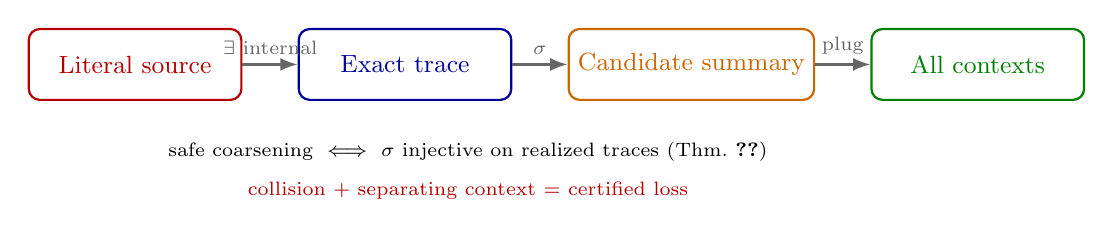
\begin{tikzpicture}[node distance=9mm and 7mm,
  box/.style={draw,rounded corners,minimum height=9mm,minimum width=27mm,align=center,font=\small,thick},
  arr/.style={-{Latex[length=2.2mm]},thick,black!60}]
\node[box,draw=red!70!black,text=red!70!black] (src) {Literal source};
\node[box,draw=blue!60!black,text=blue!60!black,right=of src] (tr) {Exact trace};
\node[box,draw=orange!80!black,text=orange!80!black,right=of tr] (sum) {Candidate summary};
\node[box,draw=green!50!black,text=green!50!black,right=of sum] (ctx) {All contexts};
\draw[arr] (src) -- node[above,font=\scriptsize]{$\exists$ internal} (tr);
\draw[arr] (tr) -- node[above,font=\scriptsize]{$\sigma$} (sum);
\draw[arr] (sum) -- node[above,font=\scriptsize]{plug} (ctx);
\node[below=4mm of tr,font=\scriptsize,align=left,xshift=8mm] {safe coarsening $\iff$ $\sigma$ injective on realized traces (Thm.~\ref{thm:realized})};
\node[below=9mm of tr,font=\scriptsize,align=left,xshift=8mm,text=red!70!black] {collision $+$ separating context $=$ certified loss};
\end{tikzpicture}
\caption{The exact decision boundary for coarsening. The trace is canonical (Theorem~\ref{thm:canonical}); the summary is conditional on the realized model class.}
\label{fig:pipeline}
\end{figure}

\section{Bounded-width composition on rooted join trees}\label{sec:junction}

\subsection{Trees, messages, and two semantics}

\begin{definition}[Rooted join tree]
Over variables $\mathrm{Var}$ with decidable equality and values $\mathrm{Val}$, a \emph{rooted join tree} is a binary tree each of whose nodes carries a bag $\beta\subseteq\mathrm{Var}$, a separator $\sigma\subseteq\beta$, a scope $\varsigma\subseteq\beta$, and a local relation $\ell(\theta,a)$ on assignments $a:\mathrm{Var}\to\mathrm{Val}$; a node is a leaf or has two children. $\mathrm{allVars}$ of a node is its bag united with the variables of its subtrees. Its \emph{width} is the maximum separator cardinality over the tree.
\end{definition}

\begin{definition}[Running intersection and local scoping]
A tree satisfies \emph{running intersection} if, recursively at every branch with bag $\beta$ and children $L,R$,
\[
\mathrm{allVars}(L)\cap(\beta\cup\mathrm{allVars}(R))\subseteq\sigma_L,\qquad
\mathrm{allVars}(R)\cap(\beta\cup\mathrm{allVars}(L))\subseteq\sigma_R .
\]
It is \emph{locally scoped} if every local relation depends extensionally only on its declared scope: assignments agreeing on $\varsigma$ receive the same verdict.
\end{definition}

\begin{definition}[Computed and global messages]
The \emph{computed message} of a node at $\theta$ to an outside assignment $o$ is defined recursively: there is an assignment $h$ agreeing with $o$ on the separator, satisfying the local relation, and (at a branch) such that both children have computed messages to $h$. The \emph{global semantic message} asserts one global assignment $g$ agreeing with $o$ on the node's separator and satisfying every local relation in the subtree.
\end{definition}

The computed message is what a local algorithm evaluates; the global message is what it is meant to mean. They are not automatically equal.

\begin{example}[Failed gluing]\label{ex:gluing}
Let a parent $P$ have children $L$ and $R$ that share a variable $x$ not routed through their separators, with $L$'s relation forcing $x=0$ and $R$'s forcing $x=1$. Each child has a computed message to any outside assignment, so the parent does. But no single global assignment satisfies both, so the global message is false. The recursive semantics is too weak precisely when a relation can inspect an out-of-scope variable or when a shared variable bypasses a separator (Figure~\ref{fig:gluing}).
\end{example}

\begin{figure}[t]
\centering
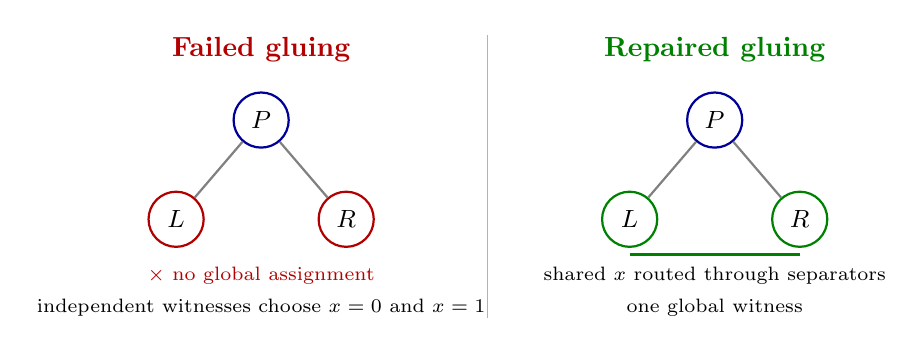
\begin{tikzpicture}[scale=0.9,every node/.style={font=\small},
  nd/.style={draw,circle,minimum size=7mm,thick}]
\begin{scope}
\node[font=\bfseries,text=red!70!black] at (0,1.6) {Failed gluing};
\node[nd,draw=blue!60!black] (p) at (0,0.6) {$P$};
\node[nd,draw=red!70!black] (l) at (-1.2,-0.8) {$L$};
\node[nd,draw=red!70!black] (r) at (1.2,-0.8) {$R$};
\draw[thick,black!50] (p)--(l) (p)--(r);
\node[text=red!70!black,font=\scriptsize] at (0,-1.6) {$\times$ no global assignment};
\node[font=\scriptsize] at (0,-2.05) {independent witnesses choose $x=0$ and $x=1$};
\end{scope}
\draw[black!30] (3.2,1.8)--(3.2,-2.2);
\begin{scope}[xshift=6.4cm]
\node[font=\bfseries,text=green!50!black] at (0,1.6) {Repaired gluing};
\node[nd,draw=blue!60!black] (p) at (0,0.6) {$P$};
\node[nd,draw=green!50!black] (l) at (-1.2,-0.8) {$L$};
\node[nd,draw=green!50!black] (r) at (1.2,-0.8) {$R$};
\draw[thick,black!50] (p)--(l) (p)--(r);
\draw[very thick,green!50!black] (-1.2,-1.3)--(1.2,-1.3);
\node[font=\scriptsize] at (0,-1.6) {shared $x$ routed through separators};
\node[font=\scriptsize] at (0,-2.05) {one global witness};
\end{scope}
\end{tikzpicture}
\caption{The central repair. Independent existential child witnesses do not glue; running intersection routes each cross-subtree shared variable through separators, and local-scope extensionality makes the splice semantically invisible.}
\label{fig:gluing}
\end{figure}

\subsection{Exact messages, substitutability, and width}

\begin{theorem}[Exact message semantics]\label{thm:message}
If a rooted join tree satisfies running intersection and is locally scoped, then at every node, parameter, and outside assignment the computed message holds iff the global semantic message holds.
\end{theorem}
\begin{proof}[Proof sketch]
Induct on the tree. At a branch with local witness $h$ and global child witnesses $g_L,g_R$, define the splice
\[
g(v)=\begin{cases}g_L(v)&v\in\mathrm{allVars}(L),\\ g_R(v)&v\in\mathrm{allVars}(R)\setminus\mathrm{allVars}(L),\\ h(v)&\text{otherwise.}\end{cases}
\]
Running intersection proves agreement on all overlaps: a variable of $L$ that also occurs in the bag or in $R$ lies in $\sigma_L$, where $g_L$ agrees with $h$, and symmetrically. Scope extensionality transports each local predicate from its own witness to $g$. The reverse direction restricts a single global witness to each recursive obligation.
\end{proof}

Removing either hypothesis reintroduces Example~\ref{ex:gluing}. The weaker dependent witness-tree semantics is provably equal to the computed message without hypotheses, but it is not the intended meaning; identifying this gap and isolating the locality condition was the central correction of the formal development.

\begin{corollary}[Separator contextual sufficiency]\label{cor:sep}
Under the hypotheses of Theorem~\ref{thm:message}, the boundary model ``computed message'' and the boundary model ``one global assignment agreeing on the separator'' have equal traces, so the recursive message may replace the literal subtree in every outside separator context.
\end{corollary}

\begin{theorem}[Bounded-width checker soundness]\label{thm:checker}
A \emph{message certificate} for a node is a relation description together with proofs that its denotation is sound and complete for the computed message. Under running intersection, local scoping, and width $\le w$, every certificate denotes exactly the global semantic message, and the node's separator has cardinality at most $w$.
\end{theorem}

The theorem is representation-neutral: a relation of low arity may still have an expensive description or an infinite domain. What is controlled is the number of exposed coordinates, which is exactly what contextual substitution requires. A rational-linear description language (finite conjunctions of atoms $\sum_i c_ix_i\lessgtr\rho$ with an explicit strictness flag, so that projection cannot silently close an open face) is provided as one instance.

\begin{corollary}[Decomposition invariance]\label{cor:decomp}
Two certified rooted join trees whose global semantic messages agree pointwise compute extensionally identical messages, regardless of shapes, bags, or elimination orders.
\end{corollary}

\begin{theorem}[Simultaneous exact replacement]\label{thm:replace}
Let $(L_i)_{i\in\mathcal I}$ be an arbitrary indexed family of \emph{exact local interfaces}: each carries its own code type, a code, a description relation, a literal relation, and a proof that the description of its code equals its literal relation pointwise. Then the conjunction of described relations equals the conjunction of literal relations, and the described and literal assemblies are indistinguishable by every boundary context.
\end{theorem}

Heterogeneity is the point: members may use genuinely different description languages, and pointwise exactness converts the conjunction of encodings into the conjunction of literal relations, after which Theorem~\ref{thm:canonical} lifts equality to all contexts.

\section{Certified instances: safe compression and certified loss}\label{sec:instances}

\subsection{The amplification price profile}

\begin{theorem}[MAF profile interface]\label{thm:maf-profile}
For networks on a common species set, the representation $N\mapsto(q\mapsto D_N(q))$ is contextually sufficient for every price-boundary context, and it composes under shared-species coupling by pointwise intersection, $D_{N_1\parallel N_2}(q)=D_{N_1}(q)\cap D_{N_2}(q)$.
\end{theorem}

\begin{theorem}[Scalar MAF loss]\label{thm:maf-loss}
The constant summary assigning the scalar $2$ to both $N_1$ and $N_2$ of Theorem~\ref{thm:scalar-noncomp} admits a loss witness: with common partner $N_1$ and parameter $q=4$, $N_2\parallel N_1$ is feasible while $N_1\parallel N_1$ is not, because $4\le 2$ is false. Hence the scalar summary is not contextually sufficient.
\end{theorem}

In the formalization the parallel composition with the fixed partner is encoded in the observable and the context type is a singleton; the instance is a faithful but schematic loss witness, and the compositional content is carried by Theorem~\ref{thm:maf-profile}. The construction is not used to weaken the positive theorem; it identifies the exact place where a popular compression loses information and directs the interface back to the price cone.

\subsection{A thermodynamic interval interface and two layered losses}

The thermodynamic material comes from a companion study \cite{thermocompanion2026} of the Strong Compatibility hypothesis of Kosc et al.~\cite{kosc2025} for families of interacting primitive autocatalytic cores in reversible mass-action networks with barrier-weighted currents $j_r=b_r(\mathbf z^{\mathrm{react}(r)}-\mathbf z^{\mathrm{prod}(r)})$. Four verdicts form a hierarchy of increasing strength for a family $F$ of oriented cores:
\begin{itemize}
\item $\MPAC(F)$: a flow $v$ with positive oriented components making every core productive;
\item $\DIR(F)$: a species potential $\mu$ with strictly positive oriented affinity on every reaction;
\item $\LCC(F)$: independent positive activities per \emph{complex} realising oriented currents that make every core productive;
\item $\MCAC(F)$: one positive species-activity vector whose monomials realise such currents (the common species-activity lift).
\end{itemize}
$\MCAC\Rightarrow\LCC$, and each step of the hierarchy is strict.

\begin{theorem}[Exact interval interface]\label{thm:triangle}
For the triangle $A\to B\to C\to mA$ with gain $m>1$ and barriers $b_0,b_1,b_2>0$, let the literal model have internal currents $(j_0,j_1,j_2)$ and boundary $q$, valid when $j_0>0$, $mj_2-j_0>0$, $j_1-j_2>0$, $j_0-j_1>0$ (positive net production of $A,C,B$) and $q=b_0\big(j_1/(b_1j_0)+j_2/(b_2j_0)\big)$. Then the trace of the literal model is exactly the open interval
\[
\frac{b_0(1/b_1+1/b_2)}{m}<q<b_0\Big(\frac1{b_1}+\frac1{b_2}\Big),
\]
so the literal current model and the interval model are contextually substitutable.
\end{theorem}

Two such triangles sharing $A\to B$ with left and right coefficients $R_L,R_R$ admit a common response iff $1/m_L<R_R/R_L<m_R$; for gain $2$ on both sides this is the window $1/2<k<2$ of the barrier ratio $k$, and the companion study proves the complete phase diagram $\MPAC\wedge\DIR\wedge(\MCAC\iff 1/2<k<2)$ for that family.

\begin{theorem}[Two strict thermodynamic losses]\label{thm:thermo-loss}
Let the control family be the two-triangle family at the interior point $k=1$ (species $A,B,C,D$; reactions $A\rightleftharpoons B$, $B\rightleftharpoons C$, $C\rightleftharpoons 2A$, $B\rightleftharpoons D$, $D\rightleftharpoons 2A$, all barriers $1$), which satisfies all four verdicts. Then:
\begin{enumerate}[label=(\roman*)]
\item (\emph{magnitude loss}) the same chemistry with right barriers $10$ satisfies $\MPAC$ and $\DIR$ but not $\LCC$; the constant two-verdict summary $(\mathsf{true},\mathsf{true})$ admits a loss witness at the observable $\LCC$;
\item (\emph{toric loss}) the two-species family $A\rightleftharpoons B$ (barrier $1$), $B\rightleftharpoons 2A$ (barrier $1$), $B\rightleftharpoons 3A$ (barrier $2$), with cores $\{A\rightleftharpoons B,\ B\rightleftharpoons 2A\}$ and $\{A\rightleftharpoons B,\ B\rightleftharpoons 3A\}$, satisfies $\MPAC$, $\DIR$, and $\LCC$ but not $\MCAC$; the constant three-verdict summary admits a loss witness at the observable $\MCAC$.
\end{enumerate}
\end{theorem}

The toric obstruction is elementary once found: left productivity forces $A>B>A^2$, hence $0<A<1$ and $B-A^3>B-A^2$, which contradicts the right core's requirement $2(B-A^3)<A-B$ against the left's $B-A^2>(A-B)/2$. Both witnesses pair a positive source theorem with a negative source theorem in the generic loss-witness structure; the summary maps are constant by construction, and the mathematical content is the paired verdicts (Figure~\ref{fig:hierarchy}).

\begin{figure}[t]
\centering
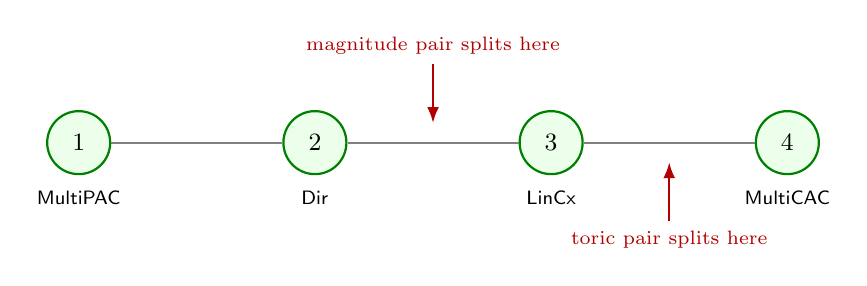
\begin{tikzpicture}[every node/.style={font=\small},
  lay/.style={draw,circle,minimum size=8mm,thick,draw=green!50!black,fill=green!8}]
\node[lay] (a) at (0,0) {1};
\node[lay] (b) at (3,0) {2};
\node[lay] (c) at (6,0) {3};
\node[lay] (d) at (9,0) {4};
\draw[thick,black!50] (a)--(b)--(c)--(d);
\node[below=2pt of a,font=\scriptsize] {$\MPAC$};
\node[below=2pt of b,font=\scriptsize] {$\DIR$};
\node[below=2pt of c,font=\scriptsize] {$\LCC$};
\node[below=2pt of d,font=\scriptsize] {$\MCAC$};
\draw[-{Latex[length=2mm]},red!70!black,thick] (4.5,1.0) -- (4.5,0.25);
\node[above,red!70!black,font=\scriptsize] at (4.5,1.0) {magnitude pair splits here};
\draw[-{Latex[length=2mm]},red!70!black,thick] (7.5,-1.0) -- (7.5,-0.25);
\node[below,red!70!black,font=\scriptsize] at (7.5,-1.0) {toric pair splits here};
\end{tikzpicture}
\caption{Two source-valid abstraction-loss cuts. Green nodes are shared positive layers; each red arrow marks the first verdict that separates the paired sources of Theorem~\ref{thm:thermo-loss}.}
\label{fig:hierarchy}
\end{figure}

\subsection{Finite Type-II passive tails are exact two-ports}

Type-II cores in the classification of \cite{blokhuis2020,nandan2026} may carry passive reversible tails. In the companion unistationarity study \cite{typeiicompanion2026} a \emph{unit chain} is built inductively: a direct edge with forward and backward rates $c,\beta>0$, or an extension of a chain by an edge $(c,\beta)$ that turns the previous right endpoint into an intermediate with degradation $d>0$. Its \emph{summary} $(c,\beta,\ell_L,\ell_R)$ is defined by the recursion, with prefix summary $(c_q,\beta_q,\ell_q,r_q)$ and $L=\beta_q+r_q+c+d>0$,
\[
c'=\frac{c_qc}{L},\qquad \beta'=\frac{\beta_q\beta}{L},\qquad \ell'_L=\ell_q+\frac{c_q(r_q+d)}{L},\qquad \ell'_R=\frac{\beta(r_q+d)}{L},
\]
starting from $(c,\beta,0,0)$. The chain-flux relation states that the internal concentrations are steady, $j_L$ leaves the left endpoint with concentration $X$, and $j_R$ enters the right endpoint with concentration $Y$.

\begin{theorem}[Exact passive-tail compression and reconstruction]\label{thm:tail}
For every finite unit chain and all boundary data $(X,Y,j_L,j_R)$: an internal steady state exists iff
\[
j_L=(c+\ell_L)X-\beta Y\quad\text{and}\quad j_R=cX-(\beta+\ell_R)Y .
\]
Whenever a steady state exists it is determined by $(X,Y)$ alone. Consequently the literal chain and its four-coefficient affine two-port have identical boundary traces and are indistinguishable by every boundary context.
\end{theorem}
\begin{proof}[Proof sketch]
Forward elimination is the known Schur-complement step. The converse is recursive: from the two compressed equations, set $Z=(c_qX+\beta Y)/L$ and $j_{\mathrm{mid}}=c_qX-(\beta_q+r_q)Z$; these satisfy the two uncompressed component equations, the node balance $j_{\mathrm{mid}}-cZ+\beta Y-dZ=0$, and the output equation, and the prefix is reconstructed by induction. Positivity of $L$ is the strictly positive total outflow of the appended intermediate.
\end{proof}

Internal degradation of a reversible chain is therefore boundary-observable \emph{only} as two endpoint leaks, which are absorbed additively into the endpoint species' degradation rates when the tail is inserted into a core. This is an exact compression in the sense of Section~\ref{sec:trace}, in contrast with the scalar MAF and the thermodynamic verdict vectors.

\section{Formal verification}\label{sec:verification}

\subsection{Environment and discipline}

All theorems are formalised in Lean~4 \cite{demoura2021} against Mathlib \cite{mathlib2020}. The environment is frozen: toolchain \lean{leanprover/lean4:v4.30.0}, Mathlib at commit \lean{c5ea0035} (full: \texttt{c5ea00351c28e24a\allowbreak fc9f0f84379aa41082b1188f}), and a Lake manifest with SHA-256 \texttt{a8df0b606ec25856\allowbreak 1c226df89856884be433c19b\allowbreak 49fb0a27335d69bb2b6e9fac}. The amplification-price receipt of Table~\ref{tab:receipts} was re-issued on the date of this manuscript after a universe generalisation of three of its modules; all other receipts match the current sources. Every module is compiled with \lean{-DwarningAsError=true}; a verification receipt records the exact command, exit code $0$, empty standard output and error, the source hash, the transitive local dependency list, the compiled artifact hash, and a fingerprint of the elaborated type of each exported declaration. No declaration uses \lean{sorry}.

\begin{table}[t]
\centering
\small
\caption{Terminal Lean declarations and receipts. Hashes are SHA-256 of the proof source file; ``deps'' counts transitive local modules materialised and strictly compiled in the receipt.}
\label{tab:receipts}
\begin{tabular}{@{}>{\raggedright\arraybackslash}p{0.22\linewidth}>{\raggedright\arraybackslash}p{0.49\linewidth}>{\raggedleft\arraybackslash}p{0.05\linewidth}>{\raggedright\arraybackslash}p{0.15\linewidth}@{}}
\toprule
Result & Declaration & deps & source hash (prefix) \\
\midrule
Section~\ref{sec:maf} (MAF calculus) & \lean{MAFComposition.mafCompositionCalculusKernel} and the nine public interfaces of \lean{proofs/MAFComposition/Main.lean} & 11 & \lean{7fc801a6...d3c2} \\
Section~\ref{sec:cs} (Thm.~\ref{thm:cs-exact}) & \lean{AutocatalyticCS.sourceDirectCSCoreEnum_exact} & 15 & \lean{0a54d083...bee8d2} \\
Section~\ref{sec:deg} (Thms.~\ref{thm:regions}--\ref{thm:partial}) & \lean{DegradationControl.sourceNetwork_arbitraryDegradationRegions}, \lean{...SpectralState}, \lean{...partialActuation_stabilizable_iff_unactuatedCertificate}, \lean{...partialActuation_spectralStabilizable_iff_unactuatedHurwitz}, \lean{...threeCycle_waterfill_global}, \lean{...arbitraryDegradationFiniteAtlas} & 15 & \lean{f773c6e9...54ed} \\
Section~\ref{sec:cic} (Thms.~\ref{thm:signed}--\ref{thm:star}) & \lean{CoreInteraction.coreInteractionCalculus}; \lean{CoreInteraction.Degradation.SourceStarData.schurLoad_spectralTrichotomy} & 35; 7 & \lean{817b43c2...fee3}; \lean{e3f82de9...8449} \\
Sections~\ref{sec:trace}--\ref{sec:junction}, \ref{sec:instances} (package) & \lean{ContextualCoreInteraction.contextualSufficiency_boundedWidth_coreInteraction} & 38 & \lean{971c2657...9661} \\
Sections~\ref{sec:trace}, \ref{sec:instances} (post-proof closure) & \lean{ContextualCoreInteraction.publication_sourceLossWitnesses}; imports \lean{trace_eq_iff_boundaryIndistinguishable}, \lean{summary_contextuallySufficient_iff_injectiveOnRealizedTraces}, \lean{computedMessage_decompositionInvariant}, \lean{simultaneous_exactLocalReplacement_contextual}, \lean{TypeIIPassiveTail.literal_passive_trace_eq} & 45 & \lean{c64ff546...81f9} \\
\bottomrule
\end{tabular}
\end{table}

\subsection{Trusted base and provenance}

The degradation, boundary-trace, and thermodynamic packages report exactly the standard axioms \lean{propext}, \lean{Classical.choice}, and \lean{Quot.sound}. The factor-interaction bundle additionally inherits three \lean{native_decide} axioms from the Example~\ref{ex:golnik33} regression it imports; these certify finite computations by the compiled evaluator rather than by the kernel and are confined to that regression. The terminal core-extraction theorem does not import that file.

The finite-dimensional Schauder fixed point used in Theorem~\ref{thm:perron} is a current-toolchain port of a public Lean development (a cube-parity Poincaré--Miranda argument followed by a simplex retraction and a compactness step); the port changed only compatibility details and the exported statement is the standard one. A broader Scarf--Brouwer development was tried first and abandoned because the port exposed roughly twenty API breaks without reducing the mathematical barrier. The gist from which the artifact was taken displayed no explicit license at retrieval, which does not affect the logical result but must be resolved before redistribution of the copied file.

Two junction-tree theorems coexist in the sources: a hypothesis-free equivalence with the dependent witness-tree semantics, and Theorem~\ref{thm:message}. Only the latter enters the public package. Likewise two checker theorems coexist and only the sound one is exported. The width-one and width-two regressions are single-leaf trees with trivial relations; they check the arithmetic, not a substantive instance.

\subsection{Experiments and their role}

Every numerical experiment in this work was a falsifier for a specific implication and was retired once it stopped discriminating hypotheses: the two-species MAF searches over coefficients in $\{0,1,2,4\}$; the nested-matching and source-enumerator regressions of Section~\ref{sec:cs}; the Type-I sweep, certificate adversaries, partial-actuation rays, Type-II$_2$ branch selection over $200$ random log-uniform parameter sets, and $500$ interval-corner samples of Section~\ref{sec:deg}; the exact-rational degradation-star preflight; and a three-element exhaustive check of Theorems~\ref{thm:canonical} and \ref{thm:realized} (all $8$ traces against all $8$ contexts; a label summary is sufficient and a cardinality summary is not). The preflights selected proof routes; none is treated as evidence for a universal theorem.

\section{Related work and novelty boundary}\label{sec:related}

\paragraph{Amplification.} The MAF is a von Neumann max--min model \cite{vonneumann1945,kemeny1956} transported to reaction networks \cite{gagrani2026maf}; its ancestry in production/price duality and theorems of the alternative \cite{gordan1873,schrijver1986} is classical and we claim none of it. Optimisation of growth bounds over subnetworks and the polyhedral geometry of autocatalytic ecosystems \cite{gagrani2024} are adjacent; recognising autocatalysis and maximising output are NP-complete in general \cite{andersen2012}. The defensible contribution is the exact operation calculus on price profiles and the two impossibility boundaries.

\paragraph{Cores.} Stoichiometric autocatalytic cores \cite{blokhuis2020}, their explicit-catalysis refinement \cite{golnik2026cores}, the bridge to RAF sets \cite{golnik2026bridging}, and unstable cores as sources of instability \cite{vassena2024} supply the semantics. The exchange-path theorem, the support-versus-edge correction, and the exact executable enumerator are new to our knowledge; the enumeration question itself is posed in \cite{golnik2026cores}.

\paragraph{Degradation.} Perron--Frobenius theory for Metzler matrices, Collatz--Wielandt characterisations, M-matrix equivalences, and projective diagonal control \cite{bermanplemmons1994,farinarinaldi2000,ofir2022} are baseline. The diluted onset model and small-degradation results are due to \cite{unterberger2022}; the classification and the open question to \cite{nandan2026}. Our contribution is the source-faithful composition from a reaction list to the spectral partition for every degradation vector, the partial-actuation theorem, and the branch diagnostics.

\paragraph{Composition and interfaces.} Exact local computation on decomposable graphical structures \cite{lauritzen1988}, bounded-width constraint satisfaction \cite{freuder1990}, acyclic database schemes \cite{beeri1983}, and factor-graph message passing \cite{kschischang2001} establish that tree-structured factorization supports exact local elimination. Behavioural systems \cite{willems2007} and categorical open reaction networks \cite{baezpollard2017} establish relational black-boxing and composition by interconnection. RAF theory \cite{hordijk2014,steel2019} supplies the structural language. We claim priority for none of these individually. The novelty claim is the conjunction: a source-faithful factorization adapter; exact all-context trace semantics; the realized-image criterion; the isolated locality condition that repairs existential witness gluing; certified bounded separator-message arity; source-level amplification, thermodynamic and Type-II instances; and a warning-free formal closure. The contribution is not a new name for belief propagation: the semantic carrier is a property-specific feasibility relation over literal source data, and the theorems establish both its maximal contextual meaning and certified cases where tempting coarsenings fail.

\section{Conclusion and open directions}\label{sec:conclusion}

Exact interfaces unify the positive and negative sides of modular proof. For the MAF, the interface is the price profile and the scalar is a certified loss. For catalyst-aware cores, the interface between an ordinary core and its extensions is a pack of exchange paths. For degradation, the interface is a positive composition, and for a star of branches it is a scalar Schur load that adds. In general, equality of exact boundary traces licenses replacement in every environment, inequality automatically supplies a separating context, and certified tree decompositions compute the same relation while exposing only bounded-arity separators.

Several directions are open and none is required by the results above. The interaction layer covers forests and one-level stars; simple-cycle gain formulas, cactus-shaped incidence graphs, and degradation trees of greater depth are the natural next targets, as is a proof-carrying rational-linear message compiler for Theorem~\ref{thm:checker}. For core extraction, output-sensitive or parameterised delay bounds, canonical anchoring to avoid duplicate work, and an end-to-end benchmark against a faithful implementation of the published complete enumeration would sharpen the practical claim. For degradation, the reducible Metzler equivalence ``Hurwitz iff strict positive supersolution'' would remove the irreducibility scope from the spectral partial-actuation corollary, and nonlinear continuation from the critical surface is a separate campaign. Finally, the MAF calculus, the degradation regions, and the trace theory together suggest a two-stage certified analysis of any proposed network edit: does the price profile prove a structural increase, and does the degradation region enlarge?

\section*{Data and code availability}

The Lean sources, verification receipts, and the deterministic experiment scripts are part of the authors' repository; the terminal declaration names and source hashes in Table~\ref{tab:receipts} identify the verified artifacts. A public release tag will accompany submission.

\bibliographystyle{unsrtnat}
\bibliography{refs}

\end{document}
